\section{Experiments}
We evaluate the application of meta-PDE to three example PDE problems: the nonlinear Poisson's Equation, the 1D Burgers’ Equation, and the Hyper-elasticity Equation. We compare Meta-PDE's performance with baseline solved by the numerical solver Fenics.
\subsection{Nonlinear Poisson Equation}
Poisson's Equation is one of the most ubiquitous equations in physics. For example, the linear Poisson's Equation calculates electrostatic or gravitational field causes by electric charges or mass particles. Since the linear Poisson's Equation can be solved analytically, we demonstrate Meta-PDE on a nonlinear Poisson problem with varying source terms, boundary conditions, and geometric domain. The nonlinear Poisson's Equation takes the form:
\begin{align*}
\nabla \cdot \left[ (1 + 0.1 u^2) \nabla u(\bm{x}) \right]&= f(\bm{x}) \quad &\bm{x} \in \Omega\\
u(\bm{x}) &= b(\bm{x}) \quad &\bm{x} \in \partial\Omega
\end{align*}
where $u \in \mathbb{R}^1$ and $\Omega \subset \mathbb{R}^2$. Using our notation from the previous section, this is equivalent to constraining the solution in the domain with an operator~${\mathcal{F}(u) = ((1 + 0.1 u^2) \nabla u) - f}$, and constraining the solution on the boundary with an operator~${\mathcal{G}(u) = u - b}$.

The domain $\Omega$ is a disc-like shape centered at the origin, defined in polar coordinates by  and the varying radius about the origin
\[
r(\theta) = r_0[1 + c_1 \cos(4\theta) + c_2 \cos(8\theta)],
\]
where the varying parameters are $c_1, c_2 \sim \mathcal{U}(-0.2, 0.2)$. The source term $f$ is a sum of radial basis functions,
\[
f(\bm{x}) = \sum_{i=1}^3 \beta_i \exp{||\bm{x} - \mu_i||_2^2},
\]
where $\beta_i \in \mathbb{R}^1$ and $\mu_i \in \mathbb{R}^2$ are both drawn from standard normal distributions. The boundary condition $b$ is a periodic function, defined in polar coordinates as
\[
b(x) = b_0 + b_1 \cos(\theta) + b_2 \sin(\theta) + b_3 \cos(\theta) + b_4 \sin(\theta),
\]
where the parameters $b_{0:4} \sim \mathcal{U}(-1, 1)$.
%Figure \todo{make fig} shows the domain, source term, and boundary conditions across several sampled PDEs.

Our MAML-based Meta-PDE model is a small NN (3 layer with layer size 64) with sinusoidal activation functions. The sinusoidal activation is initialized according to the scheme in \citet{sitzmann2020implicit}, although we replace $\omega_0 = 30.0$ in that paper with $\omega_0 = 3.0$ to avoid numerical issues when taking higher-order derivatives of a neural network's input-output function. The inner-loop (task-specific learning) takes 5 gradients steps to adapt the NN solution to a different PDE problem. We initialize the inner-loop learning rate to $1\times 10^{-4}$, and use an outer loop learning rate of $1\times 10^{-5}$. Gradients in both inner and outer loop are clipped to have maximal norm $100.0$. In the inner loop, we use vanilla SGD. In the outer loop, we use the Adam optimizer \citep{kingma2014adam}. 

Our LEAP-based Meta-PDE model uses the same architecture (3 layer with layer size 64) and sinusoidal activations between layers. The inner-loop (task-specific learning) takes 60 gradients steps. We initialize the inner-loop learning rate to $2.5\times 10^{-5}$, and use an outer loop learning rate of $5\times 10^{-5}$. Different from our MAML-based Meta-PDE model, we use  Adam optimizer \citep{kingma2014adam} for both inner loop optimizations (task-specific optimization) and the outer loop optimization (meta-learning).

We train both Meta-PDE methods with a batch size of 16 tasks. For each task, we sample 1024 sampled points on the boundary and 1024 points in the domain to evaluate the residual at each inner optimization step. 
We sample points uniformly on the domain and the boundary, which gives us strong performance. If needed, we could also divide the domain into subdomains which could lead to further variance reduction.
To sample points on the boundary, we construct an evenly spaced interval mesh of angles in $[0, 2\pi]$, add uniform noise of the size of one interval to each point, and use the points on the boundary using these angles. To sample points in the domain, we do the same but also draw random radii uniformly in $[0, r(\theta)]$. These samplers are not unbiased for non-circular shapes, but this does not change the optimal solution. 
Meta-PDE methods are implemented in Jax \citep{jax2018github}. For the MAML-based Meta-PDE method, we train for 120,000 outer-loop steps, which takes about 4 hours on one NVIDIA T4 GPUs. For the LEAP-based Meta-PDE method, We train for 55,000 outer-loop steps, which takes about 5 hours on NVIDIA T4 GPUs. All finite element baselines are implemented in FEniCS \citep{LoggMardalEtAl2012a,AlnaesBlechta2015a}. We use the Mumps linear solver backend. Figure \ref{fig:results_per_step} shows the ground truth (baseline) solution for eight PDE problems used in the validation set. The same figure also shows the MAML meta-learned initialization, which can quickly adapt to each PDE problems in five gradient steps. 

\begin{figure}[htbp]
  \centering
 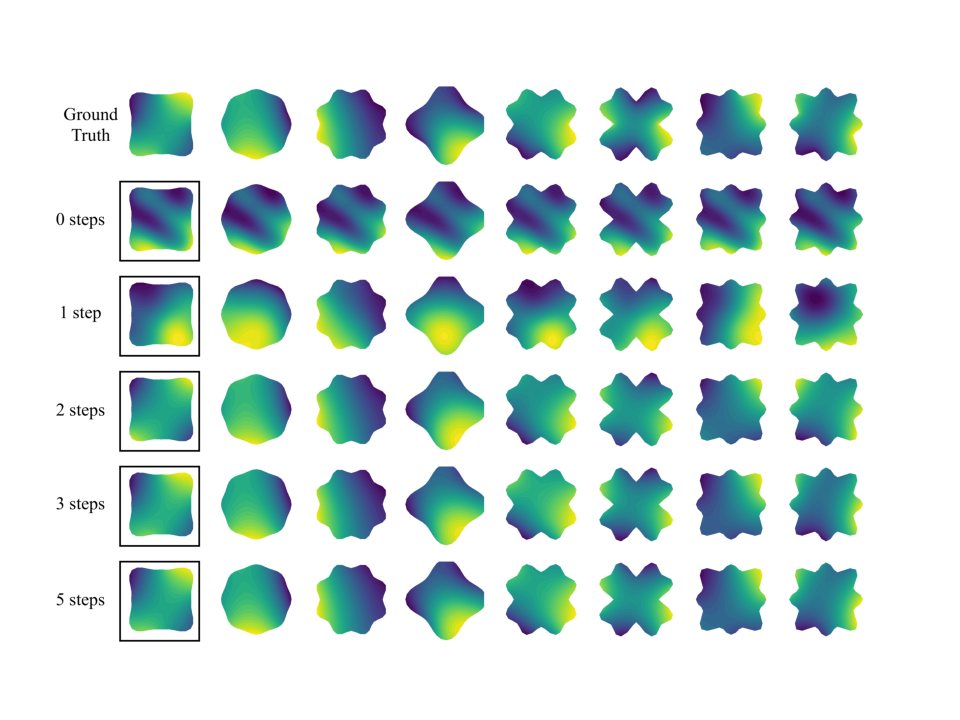
\includegraphics[width=0.8\linewidth]{figures/poisson_meta.pdf}
\caption{Solutions to nonlinear Poisson's equations with varying domains, boundary conditions and source terms. Top: ground truth finite element solution. Second row: solution represented by Meta-PDE initial neural network parameters. Third row onwards: solution after each gradient step in the Meta-PDE inner loop.}
\label{fig:results_per_step}
\end{figure}

% FENICS
% res: 1, rel_mse: 0.28237417340278625, std_rel_mse: 0.6290896534919739, time: 0.05341055989265442
% res: 2, rel_mse: 0.014543757773935795, std_rel_mse: 0.029957808554172516, time: 0.12654799222946167
% res: 3, rel_mse: 0.006523779593408108, std_rel_mse: 0.013875527307391167, time: 0.23686206340789795
% res: 4, rel_mse: 0.0011952054919674993, std_rel_mse: 0.0021807190496474504, time: 0.4497535675764084
% res: 5, rel_mse: 0.0007102875970304012, std_rel_mse: 0.0014738228637725115, time: 0.7402735650539398
% res: 6, rel_mse: 0.0003710805904120207, std_rel_mse: 0.0008687296649441123, time: 0.8322657346725464
% res: 8, rel_mse: 4.029081901535392\times 10^{-05, std_rel_mse: 5.9528952988330275\times 10^{-05, time: 1.23470838367939
% res: 10, rel_mse: 2.8872436814708635\times 10^{-05, std_rel_mse: 6.197320180945098\times 10^{-05, time: 1.8577006310224533
% res: 12, rel_mse: 5.06512105857837\times 10^{-06, std_rel_mse: 9.67413689068053\times 10^{-06, time: 2.4609854966402054

% Us
% maml_poisson_outer1en5_inner1en4_outerclip1e2_innerclip1e2
% time: 0.0022 // 0.19 s
% err: 0.00013, std 0.00027

% \begin{table}
%\begin{adjustbox}{max width=\textwidth}
%\begin{tabular}{|c|ccccc|}
% \hline
% Method & Resolution & Mean finite element DoFs & Relative MSE & Simulation time (CPU) % & Simulation time (GPU) \\
% \hline
% FEA & 1 & 15 & $0.28 \pm 0.63$ & 0.053s & N/A \\
% FEA & 2 & 53 & $0.014 \pm 0.030$ & 0.13s & N/A \\
% FEA & 3 & 85 & $0.0065 \pm 0.014$ & 0.24s & N/A \\
% FEA & 4 & 178 & $0.0012 \pm 0.0022$ & 0.45s & N/A \\
% FEA & 5 & 222 & $7.1\times 10^{-4} \pm 1.5\times 10^{-3}$ & 0.74s & N/A \\
% FEA & 6 & 324 & $3.7\times 10^{-4} \pm 8.7\times 10^{-4}$ & 0.83s & N/A \\
% FEA & 8 & 433 & $4.0\times 10^{-5} \pm 6.0\times 10^{-5}$ & 1.2s & N/A \\
% FEA & 10 & 568 & $2.9\times 10^{-5} \pm 6.2\times 10^{-5}$ & 1.9s & N/A \\
% FEA & 12 & 1246 & $5.1\times 10^{-6} \pm 9.7\times 10^{-6}$ & 2.5s & N/A \\
% FEA & 16 & 2163  & $5.1\times 10^{-6} \pm 9.7\times 10^{-6}$ & 2.92s & N/A \\
% Meta-PDE & N/A & N/A & $6.2\times 10^{-5} \pm 1.0\times 10^{-4}$  & 0.097s & 0.0022s % \\
% \hline
% \end{tabular}
% \end{adjustbox}
% \caption{
% Accuracy vs solution time for finite element methods and for meta-PDE. For FEA, a mesh % is generated with MSHR using 3x "resolution" points to define the geometry, and % "resolution" as an argument to MSHR's automeshing too.}
% \label{tbl:results}
% \end{table}
During deployment, the Meta-PDE solutions could be further improved by extending the number of "inner" training steps beyond what is specified in the Meta-PDE method. In our MAML-based Meta-PDE method for example, we first initialize the NN with the meta-learned initialization. We then perform the 5 inner-gradient steps training. After the 5 inner-gradient steps, we have the optionality to continue fitting the NN for a particular instance of PDE. The goal of further training is to fine-tune the NN to better fit a particular instance of the PDE problem. We compare the time/accuracy trade-off of our Meta-PDE method during deployment time with the FEA method. Figure \ref{fig:poisson_summary} shows the mean squared error (MSE) of each solution and solving time required for the desired accuracy. The highest-fidelity FEA method was taken as ground truth and was used to compute MSE. The MSE and solving times were evaluated using 8 held-out problems from the same distribution, and the 8 held-out problems were not used during training. Mean-squared errors are computed between the value of a given approximate solution and the value of the ground truth (highest fidelity finite element solution) at 1024 randomly sampled points within the domain. The held-out set configuration remains the same for the other two experiements below. 

% The relative mean-squared error is computed by dividing the mean-squared error by the sum of squares of solution values for the ground-truth solution.
%Figure \todo{make} shows the ground truth and finite element approximations of various fidelities for sampled test problems. 
%Figure \ref{fig:results_per_step} shows the ground truth and the Meta-PDE solution after zero through five gradient steps minimizing the variational energy for sampled test problems.\\

We see that Meta-PDE learns to output accurate solutions, and when run on the same CPU (3.6 GHz Intel Xeon Platinum 8000 series) is about $?\times - ?\times$ faster than a finite element method with similar accuracy, and about $?\times$ more accurate than a finite element method with the same computation cost. Unlike finite element models, Meta-PDE can be easily accelerated by a GPU, and on GPU we see close to $?\times$ speed up in deployment, leading to a $?\times$ speed increase over similar accuracy finite element models.

\begin{figure}[htbp]
  \centering
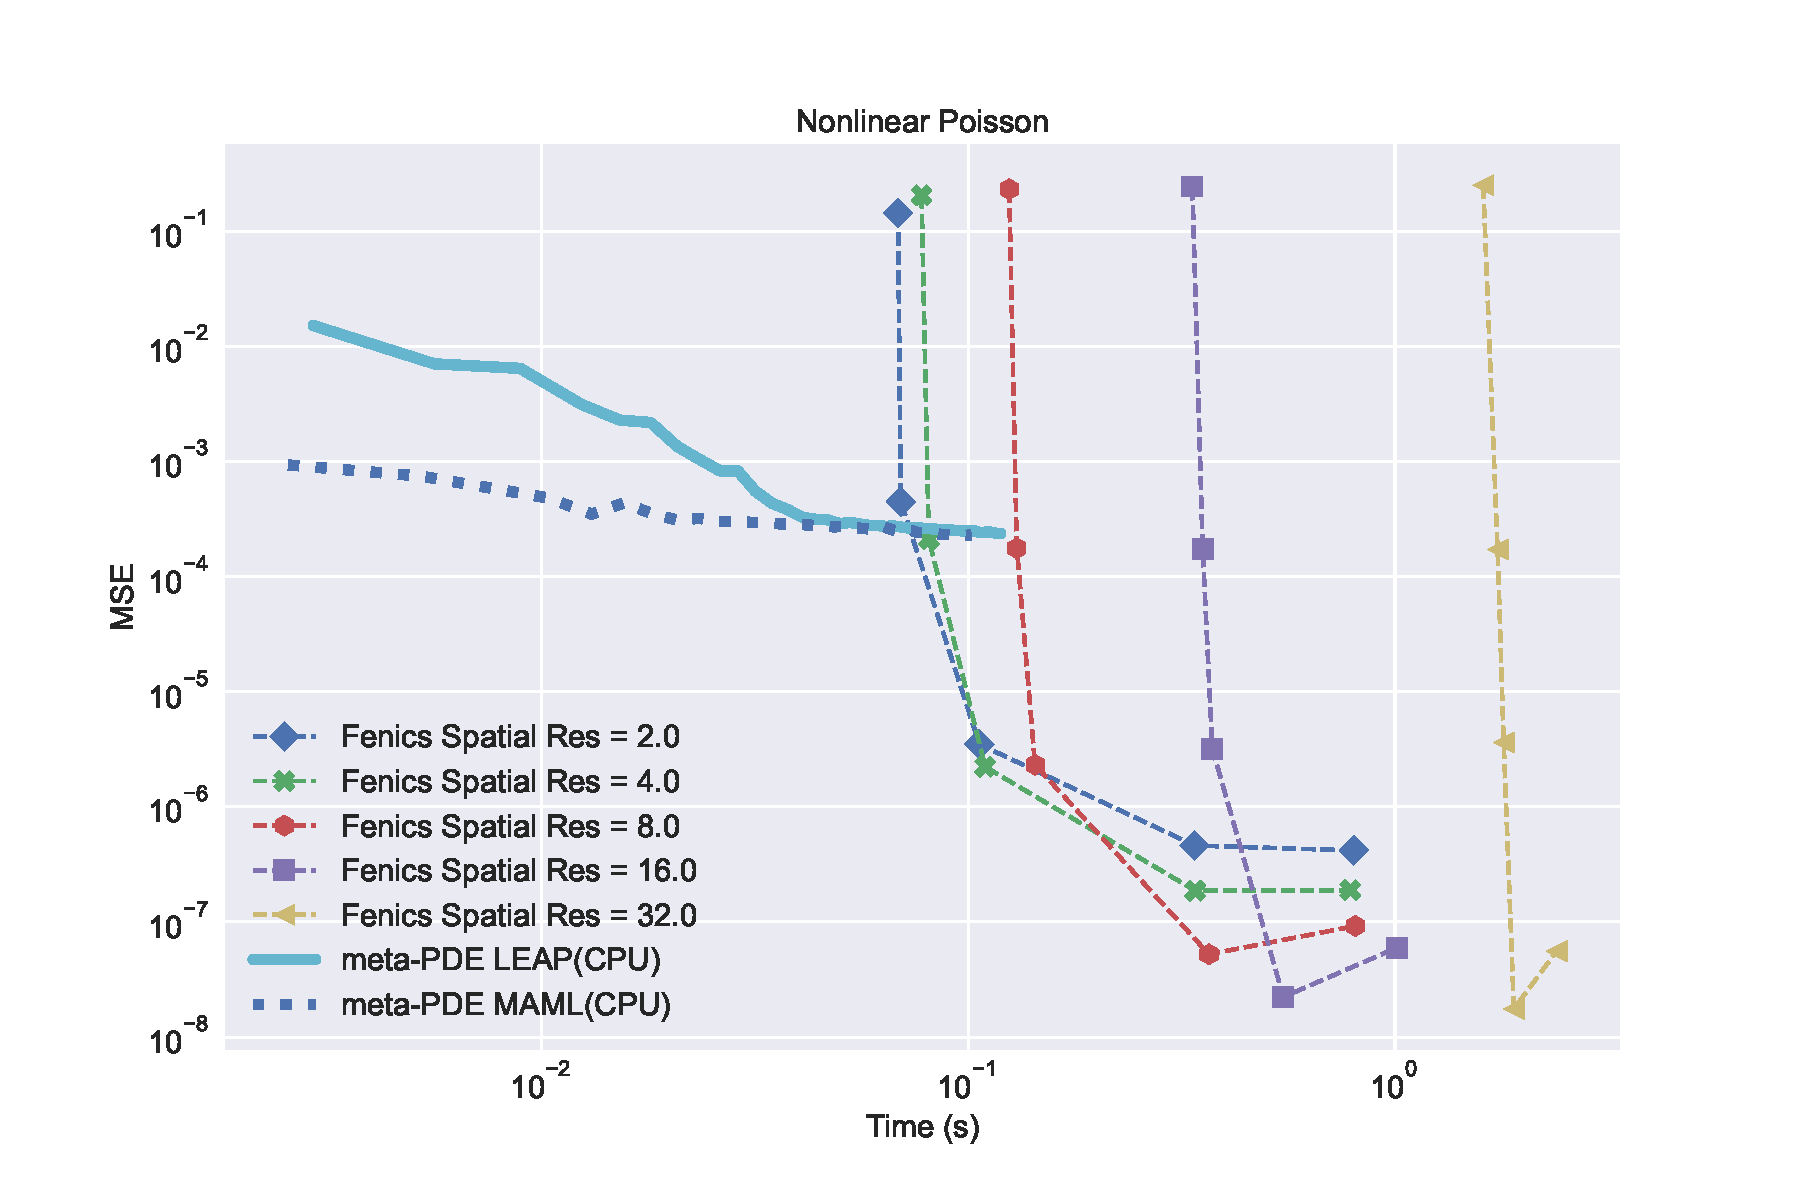
\includegraphics[width=0.8\linewidth]{figures/poisson.pdf}
\caption{MSE of each solution and the solving time required for the desired accuracy.}%
\label{fig:poisson_summary}%
\end{figure}






\subsection{Burger's Equation}
The Burger's Equation is a time-dependent PDE that models the system consisting of a moving viscous fluid. The 1D version of the equation models the fluid flow through an ideal thin pipe. The strong form of Burger's Equation is given by:
\begin{align}
    \frac{\partial u}{\partial t} + u \frac{\partial u}{\partial x} - \nu \frac{\partial ^2 u}{\partial x^2} &= 0, \quad & x \in \Omega, t \in [0, T] \\
    u(x, 0) &= u_0(x), \quad & x \in \Omega \\
    u(x, t) &= \bar{u}, \quad & x \in \partial \Omega, \in (0, T] 
\end{align}
Variable $x$ represents the spatial coordinate, and is defined on the spatial domain $\Omega$. Variable $t$ represents the temporal coordinate and the corresponding domain lives in $[0, T]$. Function $u_0(x)$ is the initial condition for the PDE and $\bar{x}$ is the boundary condition. The unknown $u(x, t)$ is the speed of the fluid, which is a function of position $x$ and time $t$. $\nu$ is the viscosity of the fluid. If the viscosity $\nu$ of the fluid is low, the fluid develops a shock wave, which is a characteristic of viscous Burger's Equation.

\begin{table}[htbp]
\caption{Neural Network hyperparameter sets for our Meta-PDE methods}
\label{tbl:hparams}
\centering
\begin{adjustbox}{max width=\textwidth}
\begin{tabular}{llllllll}
    \toprule
    PDE Problem & Meta-PDE Method & \multicolumn{6}{c}{Hyperparameters}  \\
    &  & Num. of layers & Layer Size & Activation & Inner Steps & Inner LR & Outer LR \\
    \midrule
    Nonlinear Poisson's & \multirow{3}{*}{MAML} & 3 &  \multirow{3}{*}{64} & \multirow{3}{*}{$\sin$} &  \multirow{3}{*}{5} & $1.0\times10^{-4}$ & $1.0\times10^{-5}$  \\
    Burger's &  & 8 &  &  &  & $1.0\times10^{-4} $ & $1.0\times10^{-5}$ \\
    Hyper-elasticity &  & 5 &  & &  & $1.0\times10^{-5} $ & $1.0\times10^{-5}$  \\
    \bottomrule
    Nonlinear Poisson's & \multirow{3}{*}{LEAP} & 5 & 64 & \multirow{3}{*}{$\sin$} & 60 & $2.5\times10^{-5} $ & $5.0\times10^{-5}$  \\
    Burger's &  & 5 & 64 & & 20 & $5.0\times10^{-5} $ & $5.0\times10^{-5}$  \\
    Hyper-elasticity &  & 10 & 128 &  & 20 & $1.0\times10^{-5} $ & $1.0\times10^{-5}$  \\
    \bottomrule
  \end{tabular}
\end{adjustbox}
\end{table}


\begin{table}[htbp]
\caption{\small 
Training hyperparameter set for our meta-PDE methods and corresponding training time on one NVIDIA T4 GPUs}
\label{tbl:training}
\centering
\begin{adjustbox}{max width=\textwidth}
\begin{tabular}{llllllll}
    \toprule
    PDE Problem & Meta-PDE Method & \multicolumn{6}{c}{Hyperparameters}  \\
    & & Batch Size & Sampled Points & Iterations & Training Time & Inner Optimizer & Outer Optimizer \\
    \midrule
    Nonlinear Poisson's & \multirow{3}{*}{MAML} & \multirow{3}{*}{8} & 2048 & 120,000 & 4 hrs & \multirow{3}{*}{SGD} & \multirow{3}{*}{Adam} \\
    Burger's &   &  & 1024 & 60,000 & 11 hrs  &  & \\
    Hyper-elasticity &   &  & 1024 & 180,000 & 21 hrs &  & \\
    \midrule
    Nonlinear Poisson's & \multirow{3}{*}{LEAP}  & \multirow{3}{*}{8} & 4096 & 55,000 & 5 hrs  &  \multirow{3}{*}{Adam} &  \multirow{3}{*}{Adam}\\
    Burger's &   &  & 8192 & 10,000 & 10 hrs &  & \\
    Hyper-elasticity &   &  & 1024 & 140,000 & 8 hrs &  & \\
    \bottomrule
  \end{tabular}
\end{adjustbox}
\end{table}

The NN hyperparameter set is in Table \ref{tbl:hparams} and training hyperparameter details are in Table \ref{tbl:training}. All finite element baselines are implemented in FEniCS \citep{LoggMardalEtAl2012a,AlnaesBlechta2015a}. Finite different method is applied on the time-dimension with backward explicit time stepping. For the ground truth comparison, the the time tomain $[0, T]$ is divided into time grid of size 200. We use the Mumps linear solver backend.Figure \ref{fig:burgers_per_step} shows the ground truth (baseline) solution for eight PDE problems used in the validation set. The same figure also shows the MAML meta-learned initialization, which can quickly adapt to each PDE problems in five gradient steps. 

\begin{figure}[htbp]
  \centering
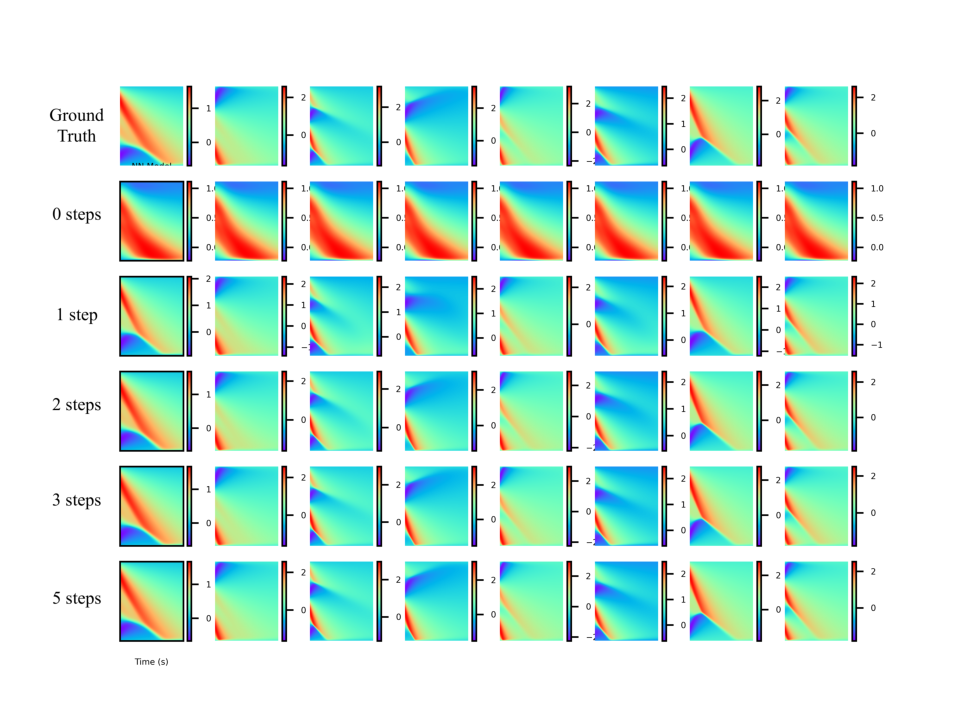
\includegraphics[width=0.8\linewidth]{figures/burgers_meta.pdf}
\caption{Solutions to Burgers's Equations with varying domains, boundary conditions and source terms. Top: ground truth finite element solution. Second row: solution represented by Meta-PDE initial neural network parameters. Third row onwards: solution after each gradient step in the Meta-PDE inner loop.}
\label{fig:burgers_per_step}
\end{figure}

Figure \ref{fig:burgers_summary} shows the mean squared error (MSE) of each solution and solving time required for the desired accuracy. We see that Meta-PDE learns to output accurate solutions, and when run on the same CPU is about $?\times - ?\times$ faster than a finite element method with similar accuracy, and about $?\times$ more accurate than a finite element method with the same computation cost. Unlike finite element models, Meta-PDE can be easily accelerated by a GPU, and on GPU we see close to $?\times$ speed up in deployment, leading to a $?\times$ speed increase over similar accuracy finite element models.

\begin{figure}[htbp]
  \centering
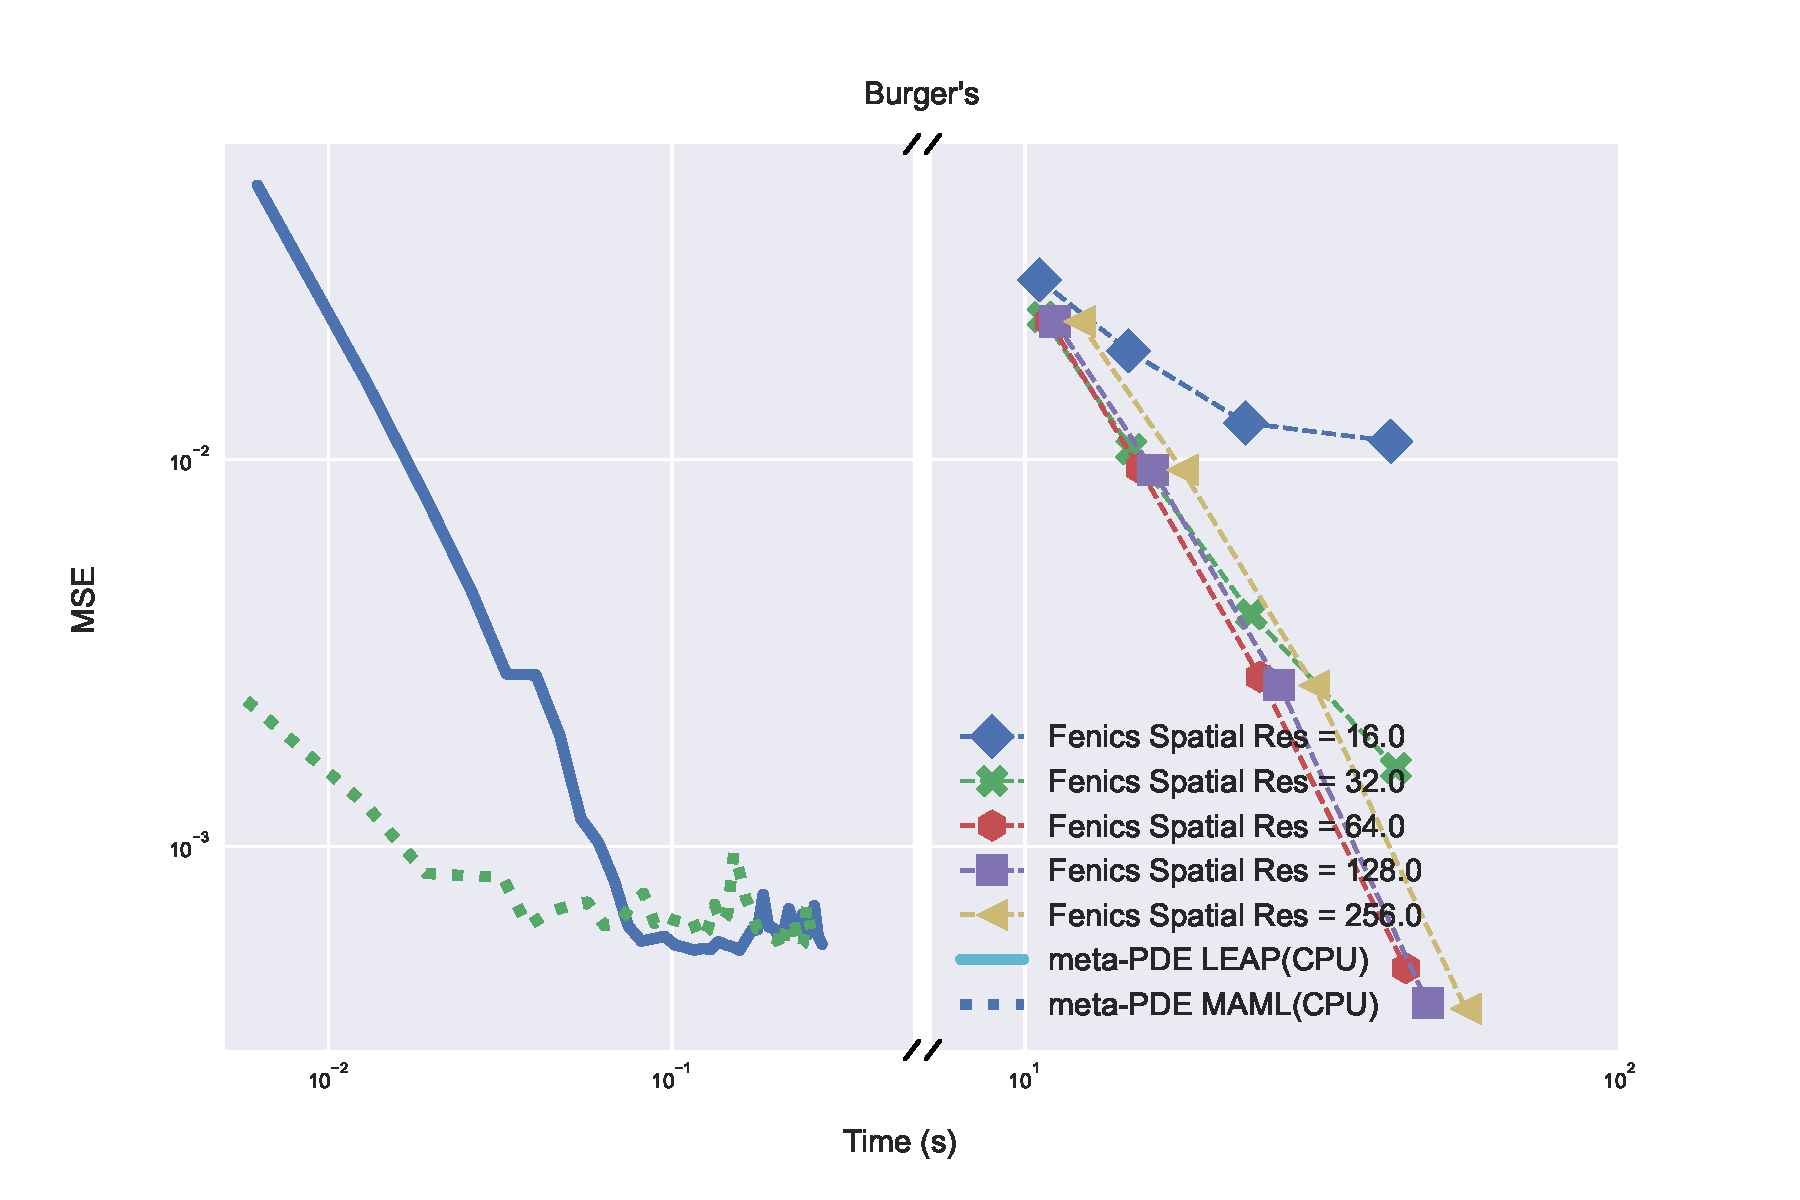
\includegraphics[width=0.8\linewidth]{figures/burgers.pdf}
\caption{MSE of each solution and the solving time required for the desired accuracy.}%
\label{fig:burgers_summary}%
\end{figure}











\subsection{Hyper-Elasticity Equation}
Hyper-elastic materials undergo large shape deformation when force is applied and the stress-strain relation for those materials are highly nonlinear. Rubber is a common example of hyper-elastic materials. the Hyper-Elasticity Equation models the deformation of those rubber-like materials under different external forces. In particular, we model a homogeneous and isotropic hyper-elasticity material under deformation when compressed uniaxially. We assume no additional body force (usually gravity) or additional traction force (usually dry friction against walls) applied to the structure. The goal is to model the final deformation displacement $u$, which maps the material position change from the initial reference position $\mathbf{X}$ to its current deformed location $\bm{x}$:
\begin{align*}
    u = \bm{x} - \mathbf{X}.
\end{align*}
The deformation gradient $F$ is defined as 
\begin{align*}
    F \equiv \frac{\partial \bm{x}}{\partial \mathbf{X}} = \frac{\partial}{\partial \mathbf{X}} \left(\mathbf{X} + u\right) = \frac{\partial \mathbf{X}}{\partial \mathbf{X}} + \frac{\partial u}{\partial \mathbf{X}} = \mathbf{I} + \frac{\partial u}{\partial \mathbf{X}}
\end{align*}
The constitutive law in continuum mechanics relates Piola-Kirchhoff stress with deformation gradient using the following relations:
\begin{align*}
    P = \frac{\partial \psi}{\partial F}
\end{align*}
where $\psi$ is the Helmholtz free energy. For Neo-Hookean hyperelasticy material, the energy is given by:
\begin{align*}
    \psi = \frac{1}{2}\lambda \left(\log(J)\right)^2 - \mu \log(J) + \frac{\mu}{2} (\mathbf{I}_c - \text{dim}).
\end{align*}
In 2-D setting, we set $dim=2$. There are two invariants in the above equation to be defined. The first is $\mathbf{I}_c \equiv tr(C) $ and $C$ is the right Cauchy-Green tensor, defined as $C = F^T F$. The second invariant is  $J \equiv \det (F)$. Substitute the two invariant into the above equation, we simply the first Piola-Kirchohoff stress $P$ into: 
\begin{align*}
    P = \frac{\partial \psi(F)}{\partial F} = \mu F \left(\lambda \ln (J) - \mu\right) F^{-T}
\end{align*}
In the absence of body and traction forces, the hyper-elastic PDE is written as
\begin{align*}
    \nabla_{\mathbf{X}} \cdot P &= 0 \quad \mathbf{X} \in \Omega \\
    \hat{u} &= g(u) \quad \mathbf{X} \in \Gamma_u \\
    P \cdot N &= T \quad \mathbf{X} \in \Gamma_T. 
\end{align*}
$N$ is the normal vector relative to $X$, the reference vector relative to the the original shape. \\
The solution $u$ to the Hyper-Elasticity Equation is also the minimizer for the Helmholtz free energy $\Pi$ of the entire system
 \begin{align*}
    u = argmin \Pi(u)
    \Pi(u) = \int_{\Omega} \psi \, d\bm{x} -\int_{\Omega} B \cdot u \, d\bm{x} -\int_{\partial \Omega} T \cdot u \, ds
\end{align*}
In the problem set-up, both body force and traction force are absent, which leads us to set $B = 0 $ and $T = 0$. The potential energy of the deformed system simplifies to: 
\begin{align*}
    \Pi(u) = \int_{\Omega} \psi(u) \, d\bm{x}
\end{align*}
There are two different approaches to encode the loss function for the Hyper-Elasticity Equation. First, one could directly minimize the residual term in the original strong form, the same approach as we have done for the nonlinear Poisson's Equation and for the Burger's Equation. For example, \citep{abueidda2021meshless} has used the first approach to encode the loss function for PiNN. Alternatively, one can minimize the Helmholtz free energy of the system and find the corresponding minimizer $u$. We will use the second approach to solve the Hyper-Elasticity Equation. 

We consider the deformation of a two-dimensional porous hyper-elastic material under compression. Their material properties could be very different from their solid counterparts. Because of these interesting differences, the hyper-elastic behavior of porous structures is an active field of research in material science \citep{overvelde2014relating, overvelde2012compaction}. Following the problem setup in \citep{overvelde2014relating}, we use the following parametrized equations to model the shape of the pores:
\begin{align*}
    x_1 &= r(\theta)\cos \theta, \, x_2 = r(\theta)\sin \theta \\
    r(\theta) &= r_0 \left[ 1 + c_1 \cos(4 \theta) + c_2\cos(8\theta)\right] \\
    r_0 &= \frac{L_0 \sqrt{2\phi_0}}{\sqrt{\pi \left(2 + x_1^2 + x_2^2\right)}}
\end{align*}
$\phi_0$ is the initial porosity of the structure, and is fixed to be 0.46 in our experiment setup. $L_0$ is the initial center-to-center distance between neighboring pores. We set the parameter pair $(c_1, c_2)$ to be both uniformly chosen between $[-0.1, 0.1]$. Fixing porosity $\psi_0$ and the distance between pore centers $L_0$, the shape of the pore affects the deformation behavior of the macroscopic structure. Figure \ref{fig:hyper-elasticity-example} shows three deformation example seen in experiments. 
\begin{figure}[H]
  \centering
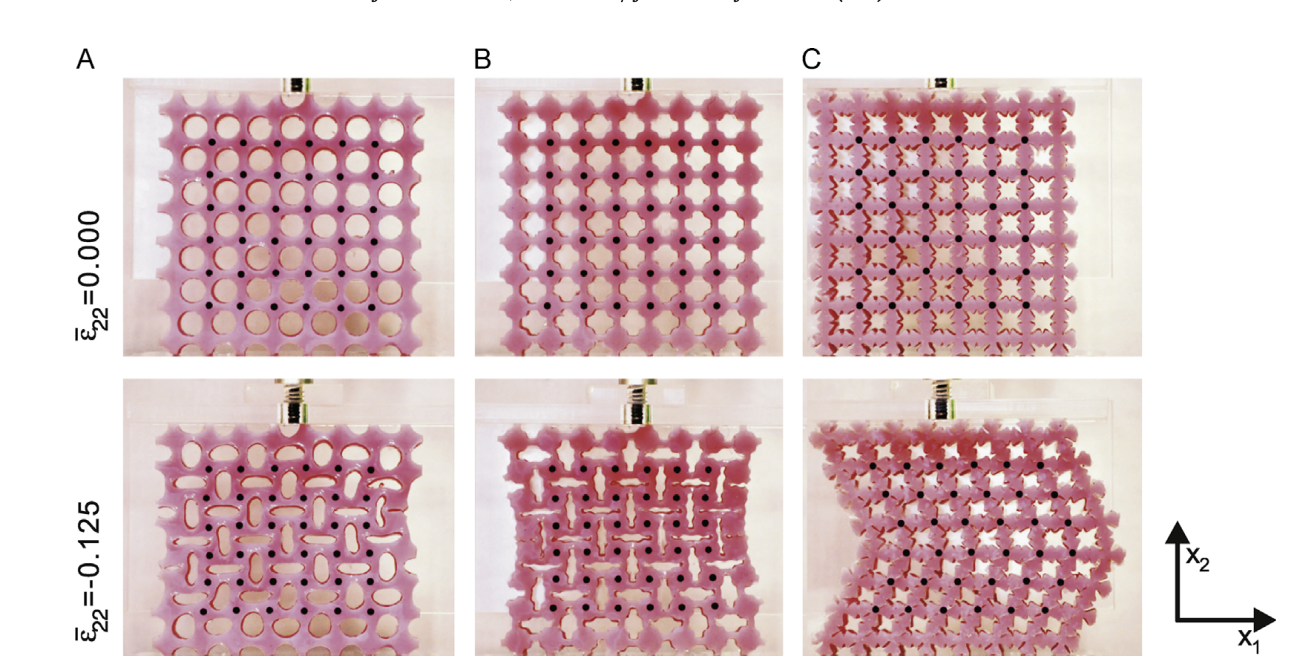
\includegraphics[width=0.8\linewidth]{figures/hyper_elasticity_example.png}
\caption{Experimental images of three structures with pores shapes loaded under uniaxial compression. All structures are characterized by 50$\%$ porosity and the same strain is applied from above down. The shape of the pores affect the deformation behavior of the structure.
Figure: \citet{overvelde2014relating}.}
\label{fig:hyper-elasticity-example}%
\end{figure}

The NN hyperparameter set is in Table \ref{tbl:hparams} and training hyperparameter details are in Table \ref{tbl:training}. Figure \ref{fig:hyperelasticity_per_step} shows the ground truth (baseline) solution for eight PDE problems used in the validation set. The same figure also shows the MAML meta-learned initialization, which can quickly adapt to each PDE problems in five gradient steps. 

\begin{figure}[htbp]
  \centering
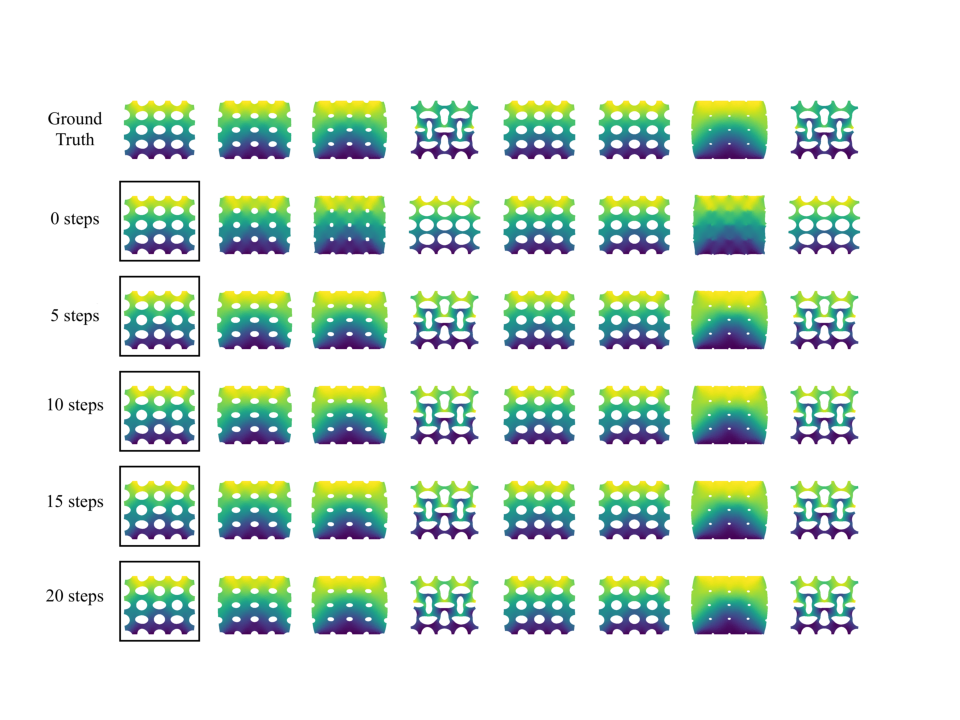
\includegraphics[width=0.8\linewidth]{figures/hyper_elasticity_circle_meta.pdf} 
\caption{Solutions to Hyper-Elasticity Equations with varying domains. Top: ground truth finite element solution. Second row: solution represented by Meta-PDE initial neural network parameters. Third row onwards: solution after each gradient step in the Meta-PDE inner loop.}
\label{fig:hyperelasticity_per_step}
\end{figure}

Figure \ref{fig:hyperelasricity_summary} shows the mean squared error (MSE) of each solution and solving time required for the desired accuracy. We see that Meta-PDE learns to output accurate solutions, and when run on the same CPU is about $?\times - ?\times$ faster than a finite element method with similar accuracy, and about $?\times$ more accurate than a finite element method with the same computation cost. Unlike finite element models, Meta-PDE can be easily accelerated by a GPU, and on GPU we see close to $?\times$ speed up in deployment, leading to a $?\times$ speed increase over similar accuracy finite element models.

\begin{figure}[htbp]
  \centering
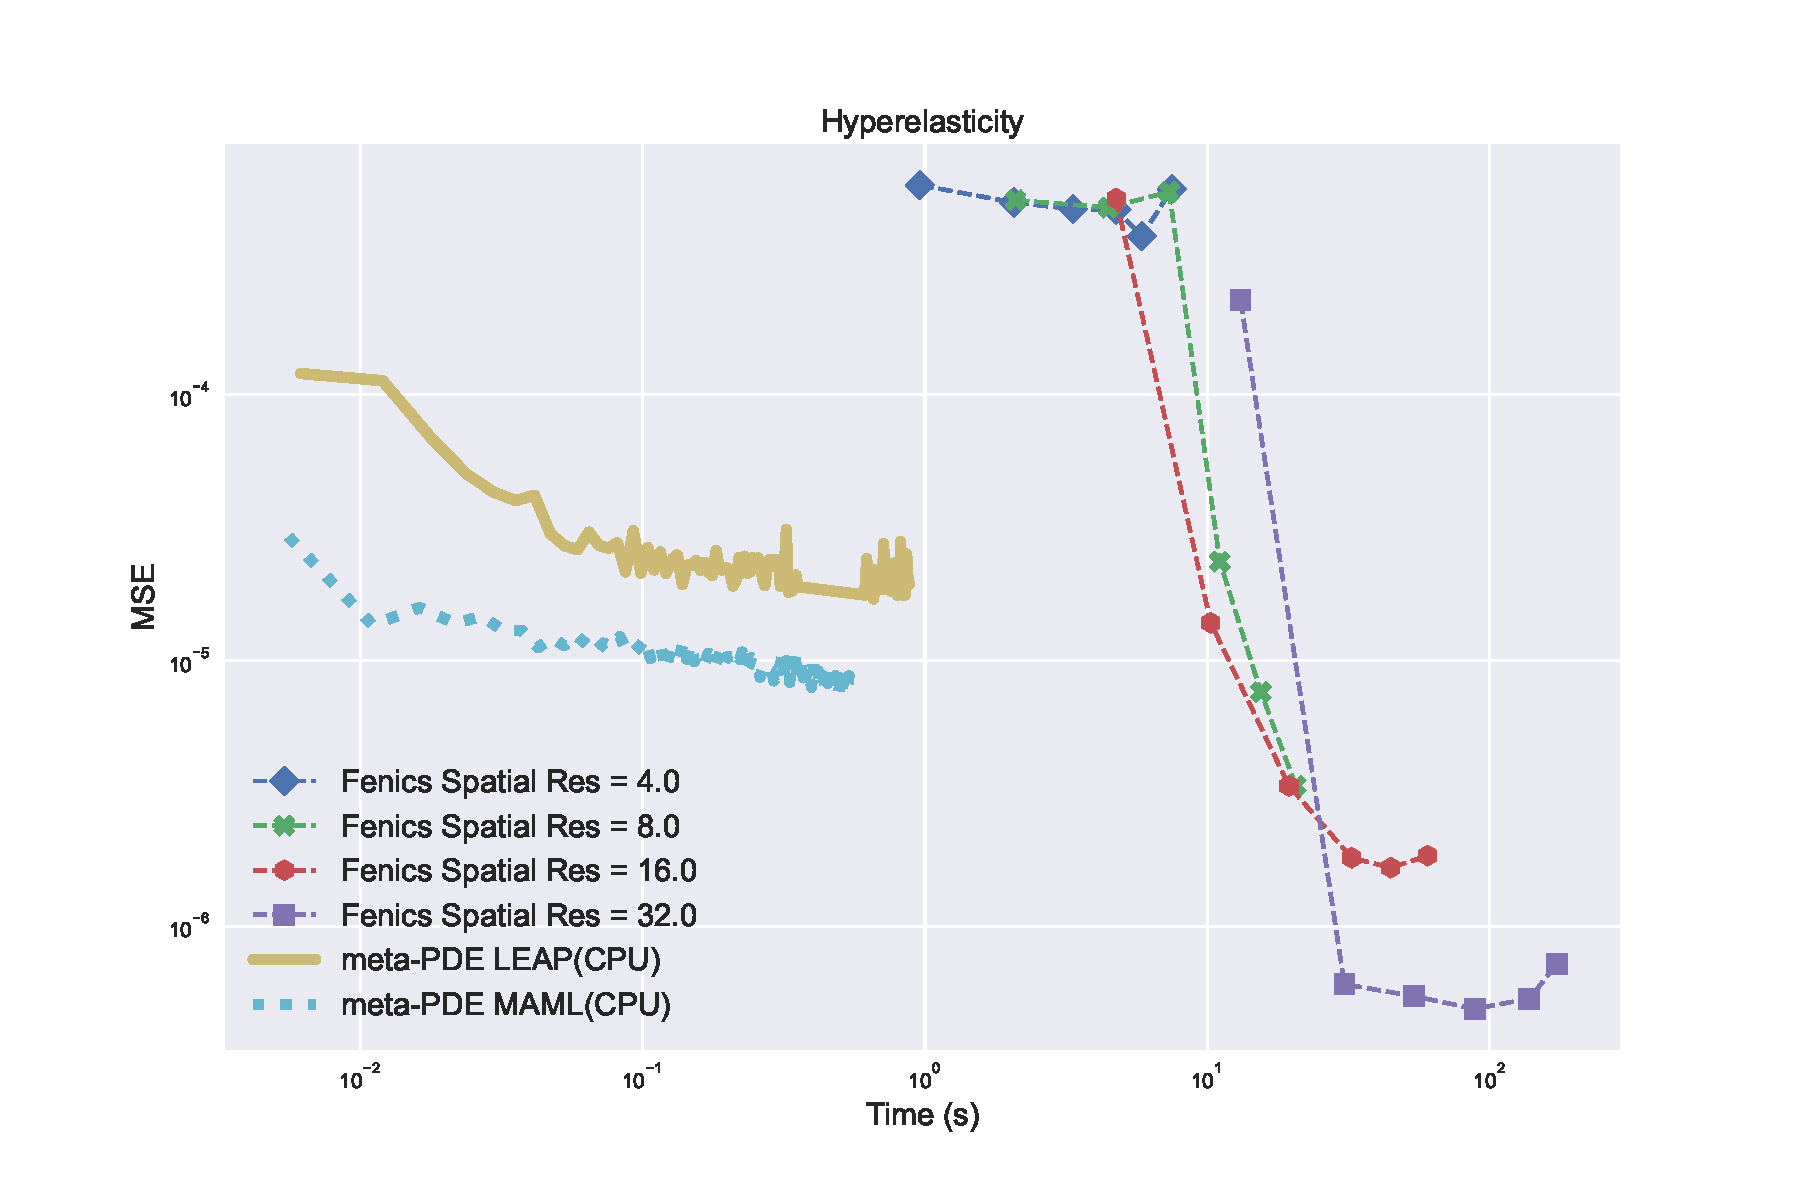
\includegraphics[width=0.8\linewidth]{figures/hyperelasticity.pdf} 
\caption{MSE of each solution and the solving time required for the desired accuracy.}%
\label{fig:hyperelasricity_summary}%
\end{figure}
